%%%%%%%%%%%%%%%%%%%%%%%%%%%%%%%%%%%%%%%%%
% The Legrand Orange Book
% LaTeX Template
% Version 2.1.1 (14/2/16)
%
% This template has been downloaded from:
% http://www.LaTeXTemplates.com
%
% Original author:
% Mathias Legrand (legrand.mathias@gmail.com) with modifications by:
% Vel (vel@latextemplates.com)
%
% License:
% CC BY-NC-SA 3.0 (http://creativecommons.org/licenses/by-nc-sa/3.0/)
%
% Compiling this template:
% This template uses biber for its bibliography and makeindex for its index.
% When you first open the template, compile it from the command line with the 
% commands below to make sure your LaTeX distribution is configured correctly:
%
% 1) pdflatex main
% 2) makeindex main.idx -s StyleInd.ist
% 3) biber main
% 4) pdflatex main x 2
%
% After this, when you wish to update the bibliography/index use the appropriate
% command above and make sure to compile with pdflatex several times 
% afterwards to propagate your changes to the document.
%
% This template also uses a number of packages which may need to be
% updated to the newest versions for the template to compile. It is strongly
% recommended you update your LaTeX distribution if you have any
% compilation errors.
%
% Important note:
% Chapter heading images should have a 2:1 width:height ratio,
% e.g. 920px width and 460px height.
%
%%%%%%%%%%%%%%%%%%%%%%%%%%%%%%%%%%%%%%%%%

%----------------------------------------------------------------------------------------
%	PACKAGES AND OTHER DOCUMENT CONFIGURATIONS
%----------------------------------------------------------------------------------------

\documentclass[11pt,fleqn]{book} % Default font size and left-justified equations

\usepackage{ifthen} 
\newboolean{VersionProf}
\setboolean{VersionProf}{false}

\usepackage{wasysym}
\usepackage{esint} % various fancy integral symbols
\usepackage{tikz}
\usepackage{tikz-3dplot}
\usepackage{pgfplots}
\pgfplotsset{compat=1.17}
\usetikzlibrary{patterns}
\usepackage{tkz-euclide} 
\usepackage{mathtools}
\usepackage{xurl}
\usepackage[version=4,arrows=pgf-filled,
textfontname=sffamily,
mathfontname=mathsf]{mhchem}
\usepackage{gensymb}
\usepackage{tabularray}
\usepackage{csquotes}
\usepackage{amsmath}
\usepackage{amsfonts}

\usepackage[french]{babel}
\usepackage{dingbat}

\usepackage{environ}
\usepackage{wrapfig}

\NewEnviron{solution}{%
    \ifthenelse{\boolean{VersionProf}}{\begin{solutionA}
        \BODY%*
        \end{solutionA}
    }{%
        \relax%
    }%
}%

\usetikzlibrary {arrows.meta} 

\newcommand{\degC}{{\degree}C}
\newcommand{\dd}{\mathrm{d}}
\newcommand{\div}{\mathrm{div}}
\newcommand{\rot}{\vv{\mathrm{div}}}
\newcommand{\grad}{\vv{\mathrm{grad}}}
\NewCommandCopy{\amshbar}{\hbar}

\tikzset{
    support/.style={
        pattern=north east lines,
        draw=none,
        minimum width=0.3,
        minimum height=0.6
    }
    ,>=latex
}

\usepackage[d]{esvect}

%SPECIFIC TO THIS CHAPTER
\usepackage{physics}
\usepackage{ifthen}
\usepackage[outline]{contour} % glow around text
\usetikzlibrary{calc} % for pic
\usetikzlibrary{angles,quotes} % for pic
\usetikzlibrary{patterns}
\tikzset{>=latex} % for LaTeX arrow head
\contourlength{1.2pt}

\colorlet{myred}{red!65!black}
\definecolor{myred}{RGB}{127,0,255}
\tikzstyle{ground}=[preaction={fill,top color=black!10,bottom color=black!5,shading angle=20},
                    fill,pattern=north east lines,draw=none,minimum width=0.3,minimum height=0.6]
\tikzstyle{mass}=[line width=0.6,myred,fill=myred!40,rounded corners=1,
                  top color=myred!40,bottom color=myred!20,shading angle=20]
\tikzstyle{rope}=[myred!30,line width=1.2,line cap=round] %very thick

% FORCES SWITCH
\tikzstyle{force}=[->,myred,ultra thick,line cap=round]
\tikzstyle{Fproj}=[force,myred!60]
\newboolean{showforces}
\setboolean{showforces}{true}
%----------------------------------------------------------------------------------------

\input{structure} % Insert the commands.tex file which contains the majority of the structure behind the template

\begin{document}

%----------------------------------------------------------------------------------------
%	TABLE OF CONTENTS
%----------------------------------------------------------------------------------------

%\usechapterimagefalse % If you don't want to include a chapter image, use this to toggle images off - it can be enabled later with \usechapterimagetrue

\chapterimage{a_boy_and_his_atom.png} % Table of contents heading image

%\pagestyle{empty} % No headers

%\tableofcontents % Print the table of contents itself

%\cleardoublepage % Forces the first chapter to start on an odd page so it's on the right

%\pagestyle{fancy} % Print headers again



%\part{\'{E}lectromagnétisme}

\setcounter{chapter}{10}

\chapter{Dualité onde-corpuscule}

\section{Introduction historique}

\textit{Cette introduction a pour but de vous expliquer comment la théorie de la mécanique quantique est née, et de présenter les raisons qui ont amené les scientifiques à proposer une description ondulatoire de la matière. Les parties historiques, en particulier les dispositifs expérimentaux utilisés, ne sont pas à connaître.}

A la fin du XIXe siècle, en Europe, la physique se porte à merveille. Les théories de l'optique, de l'électromagnétisme, de la thermodynamique et de la mécanique newtonienne permettent de décrire un grand nombre de phénomènes naturels, et ont joué un rôle important dans la révolution industrielle. 

Cependant, quelques observations viennent alors bousculer la compréhension que l'on a de certains concepts fondamentaux que l'on a en physique : la lumière, la matière, la nature d'une onde.

\subsection{Découvertes de particules}

Jusqu'à cette époque, la description de la matière en physique se faisait de manière exclusivement continue, à partir de variables telles que la masse volumique $\mu$, la densité volumique de charge $\rho$, la densité volumique de courant $\vv j$, la température $T$, la pression $p$... On connaissait l'existence des atomes, mais on cherchait à leur donner une description continue (pour plus de détails, consulter le DM d'électromagnétisme sur les modèles de l'atome). Cependant, on commence à découvrir que dans les atomes, la charge n'est pas uniformément répartie, mais elle est concentrée dans une petite partie de l'espace :
\begin{itemize}
	\item En 1897, Thomson découvre l'électron, concluant une série de travaux de nombreux scientifiques ayant étudié les rayons cathodiques. On découvre alors que la masse de l'électron et sa charge sont toujours les mêmes : il s'agit d'une propriété fondamentale. Par ailleurs, les électrons semblent émis par tout type de matière, il s'agit donc probablement d'une brique constitutive des atomes.
	\item Puis en 1911, Rutherford découvre le noyau des atomes, à partir de la déviation de particules $\alpha$ par des noyaux d'Hélium (cf DM d'électrostatique).
\end{itemize}
On comprend alors que la matière est composée de "grains" élémentaires, les \textit{particules}, qui présentent des propriétés fondamentales telles que leur masse et leur charge électrique. Cela ne pose pas de problème a priori, puisqu'il est toujours possible de se ramener à une description continue en utilisant le fait que l'on a un grand nombre de particules dans un volume mésoscopique de matière. Par ailleurs, les lois de la physique newtonienne sont parfaitement applicables à ces particules ponctuelles.

\subsection{Caractère corpusculaire de la lumière}

\subsubsection{Le rayonnement du corps noir}

Les réelles interrogations arrivent avec d'autres résultats. Un des échecs de la physique classique, bien connu à l'époque, est son incapacité à expliquer le rayonnement produit par un corps chauffé. Comme nous l'avons vu plus tôt dans l'année, plus un corps est chaud, plus il émet un rayonnement intense, à une longueur d'onde petite. Cependant, la physique classique est incapable d'expliquer la présence de ce pic et prédit un rayonnement qui contient une énergie infinie aux faibles longueurs d'onde. C'est ce qu'on appelle la \textit{catastrophe ultraviolette}. En 1900, Planck fait une hypothèse saugrenue : il introduit une constante $h$ dans ses calculs telle que l'énergie du rayonnement lumineux est quantifiée d'une manière proportionnelle à la fréquence : $E = n h \nu$. Son but était de faire le calcul par une autre méthode, puis de faire tendre $h$ vers 0. Or, il constate que le résultat qu'il obtient, la loi de Planck, ajuste parfaitement les observations... mais sans faire tendre $h$ vers 0 ! Il obtient la loi de Planck donnant la densité volumique d'énergie du rayonnement émis par un corps noir chauffé :
\begin{equation}
	u(\nu) = \dfrac{8 \pi \nu^2}{c^3} \cdot \dfrac{h \nu}{\left( e^{\frac{h \nu}{k_B T}}-1 \right)}
\end{equation}
où $\nu$ est la fréquence de l'onde, $c$ la vitesse de la lumière, $T$ la température et $k_B$ la constante de Boltzmann. L'ajustement avec les observations donne la valeur de la constante de Planck : $h = 6.63 \times 10^{-34}$\,J$\cdot$s.

\begin{figure}[htbp]
	\centering 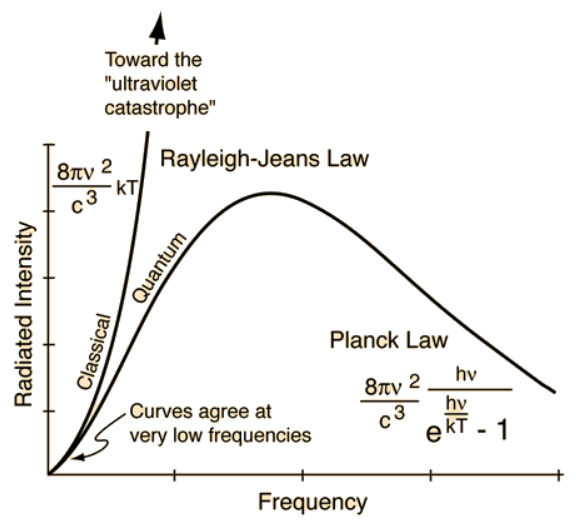
\includegraphics[width=0.5\linewidth]{loi_de_planck.png}
	\caption{Loi de Rayleigh-Jeans (issue de l'électromagnétisme classique) et loi de Planck. Source : Physics Stackexchange.}
\end{figure}

Cette quantification de l'énergie est curieuse. Si elle est essentiellement vue comme un artifice de calcul, son interprétation va changer avec le résultat de plusieurs expériences. 

\subsubsection{L'effet photoélectrique}

L'effet photoélectrique est un phénomène physique connu depuis déjà longtemps (Becquerel en 1839 puis Hertz en 1887) : certains métaux semiconducteurs libèrent des électrons lorsqu'ils sont éclairés, et sont ainsi une source de courant électrique. Nous avons d'ailleurs vu plusieurs fois en TP cet effet : il est à la base de l'utilisation d'une photodiode pour mesurer une intensité lumineuse. Ainsi, un apport sous forme énergétique permet d'extraire des électrons du métal.

On pourrait s'attendre à ce que le nombre d'électrons extraits soit proportionnel à l'énergie reçue par le métal, donc à l'intensité lumineuse appliquée. Or, on constate expérimentalement qu'il existe un effet de seuil en longueur d'onde :
\begin{itemize}
	\item En-dessous d'une fréquence critique $\nu_c = c/\lambda_c$, aucun électron n'est extrait ;
	\item Au contraire, lorsque $\nu \ge \nu_c$, l'effet photoélectrique se manifeste et le nombre d'électrons extraits n'augmente pas si la fréquence est augmentée. En revanche, l'énergie cinétique des électrons extraits augmente.
\end{itemize}

\begin{figure}[htbp]
	\centering 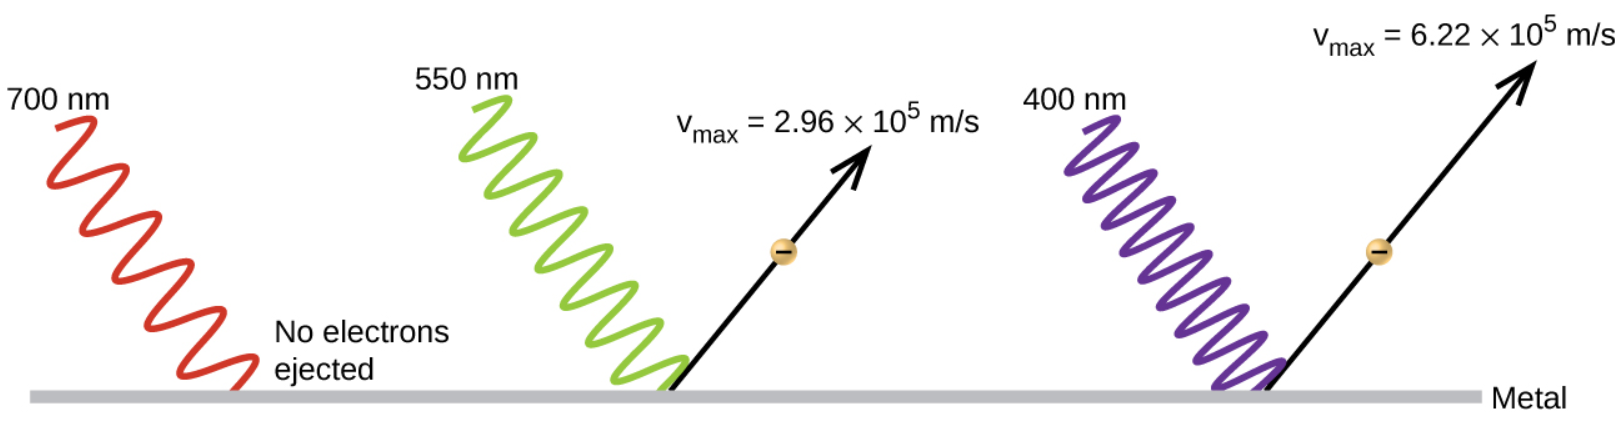
\includegraphics[width=\linewidth]{effet_photoelectrique.png}
	\caption{Effet photoélectrique sur du potassium. Les électrons sont extraits uniquement en-dessous d'une longueur d'onde limite. Source : université du Wisconsin.}
\end{figure}

Il s'agit d'un effet "tout ou rien" : soit la fréquence de l'onde est suffisante pour extraire les électrons, soit elle ne l'est pas. C'est Einstein, en 1905\footnote{La même année, il a publié deux autres articles qui ont posé les fondements de la théorie de la relativité restreinte et de la physique statistique, respectivement. L'année 1905 est souvent qualifiée de \textit{Annus mirabilis}. Le travail d'historiens à partir de plusieurs sources de l'époque a montré que Mileva Maric a travaillé en collaboration avec Einstein à la rédaction de ces articles ; en particulier elle aurait contribué à la mise en forme mathématique des idées physiques proposées par Einstein. Il y a débat sur l'ampleur de sa contribution, mais plusieurs auteurs estiment qu'elle aurait dû être co-autrice des articles portant sur la relativité restreinte et l'effet photoélectrique.}, qui propose une interprétation de cette expérience en faisant le lien avec le calcul réalisé par Planck cinq ans plus tôt : en supposant que la lumière est transporté par des particules, les photons, dont l'énergie est proportionnelle à la fréquence : on explique directement les observations : soit l'énergie du photon est supérieure au travail à apporter pour extraire l'électron, soit elle ne l'est pas. L'hypothèse formulée dans l'article se confirme au fil des années et donne naissance à la loi de Planck-Einstein :
\begin{theorem}[Loi de Planck-Einstein]
	La lumière est transportée par des particules élémentaires, les photons, qui sont caractérisés par leur fréquence $\nu$ et se déplacent à la vitesse de la lumière $c$. Chaque photon transporte une énergie $E$ proportionnelle à sa fréquence :
	\begin{equation}
		E = h \nu = \frac{h c}{\lambda}
	\end{equation}
	où $h = 6.63 \times 10^{-34}$\,J$\cdot$s est la constante de Planck.
\end{theorem}

\subsubsection{Autres expériences}

L'interprétation quantique de l'effet photoélectrique sera confirmée plus tard par des expériences plus sophistiquées spécifiquement conçues pour établir la nature corpusculaire de la lumière. On peut notamment citer l'expérience de Millikan (1916), et plus récemment le travail d'équipes françaises, notamment à l'Ecole Normale Supérieure de Paris, qui ont permis de mettre en évidence sans équivoque la quantification de l'énergie électromagnétique.

Les résultats de toutes ces expériences sont une détonation dans le monde de la physique classique. Si la lumière était corpusculaire, elle devrait être décrite par des principes similaires à la mécanique Newtonienne, qui ne permet pas de rendre compte des phénomènes de diffraction et d'interférences en optique. Ces phénomènes, en revanche, sont bien expliqués par l'électromagnétisme et l'optique. La lumière est-elle une onde ou une particule ? Force est de constater que les deux descriptions sont nécessaires pour expliquer les observations... mais cela n'est pas réellement satisfaisant, car il n'existe aucun cadre conceptuel pour les unifier.

\subsection{Caractère ondulatoire de la matière}

\subsubsection{Diffraction des électrons}

On sait maintenant que la lumière se décrit par une dualité onde-particule. Qu'en est-il de la matière ? On l'a toujours considérée comme une particule, mais en 1923, de Broglie remarque des analogies formelles entre les propriétés d'optique (telles que le principe de retour inverse de la lumière) et des propriétés de mécanique analytique (hors programme en MP). Ces analogies sont similaires aux analogies que l'on a pu faire entre électrostatique et gravitation au début de l'année, et elles lui permettent de définir une longueur d'onde pour une particule de masse $m$, appelée longueur d'onde de de Broglie :
\begin{equation}
	\lambda_{\mathrm{dB}} = \frac{h}{p}
\end{equation}
où $p = m v$ est la quantité de mouvement de la particule. Ses travaux sont repris en 1925 par Davisson et Germer, qui ont réussi à diffracter des électrons par un réseau cristallin. Le réseau cristallin a un pas qui est similaire à la longueur d'onde de de Broglie des électrons, et ainsi on observe des pics de diffraction dans certaines directions angulaires. C'est la première preuve expérimentale de la nature ondulatoire de la matière.

\subsubsection{Vers une nouvelle description des particules}

En 1989, des expériences similaires ont été reproduites avec un dispositif similaire aux fentes d'Young par une équipe japonaise : en envoyant un par un des électrons, on observe des franges apparaître sur un écran où l'on mesure les impacts d'électrons.

\begin{figure}{htbp}
	\centering 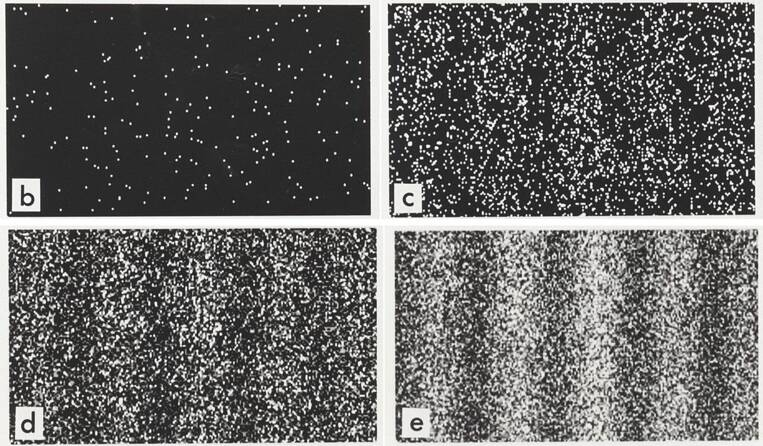
\includegraphics[width=0.8\linewidth]{Double_slit_Tonomura.jpg}
	\caption{Résultats d'une expérience dans laquelle les électrons sont envoyés un à un à travers des bifentes. Source : Tonomura (1989).}
\end{figure}

Comment interpréter ce résultat ? On pourrait penser que les interférences observées sont liées à des électrons qui ont traversé les deux fentes d'Young simultanément, puis ont interagi. Mais ce n'est pas le cas, car les électrons sont envoyés un par un dans le dispositif. Ainsi, \textbf{les interférences se produisent même lorsqu'on considère le passage d'un électron unique} : l'électron est sensible à la présence des deux fentes à la fois. L'électron ne peut donc pas être décrit pas un point matériel. Par ailleurs, si l'on place un détecteur pour savoir par quelle fente l'électron est passé, les interférences disparaissent.

\section{Fondements de la mécanique quantique ondulatoire}

\subsection{Fonction d'onde}

\subsubsection{Densité de probabilité de présence}


Nous voulons adopter une description des objets matériels qui rende compte à la fois de leur aspect corpusculaire et de leur aspect ondulatoire, non localisé. Pour cela, on travaille avec la notion de densité de probabilité de présence. On distingeura le cas général, en trois dimensions, et le cas unidimensionnel, auquel nous nous restreindrons pour la plupart des applications.

\paragraph{Cas général (3D)}

\begin{definition}[Densité de probabilité 3D]
	On définit la densité de probabilité de présence d'une particule, notée $\rho^{3D}_\mathbb{P}(M,t)$, comme un champ scalaire tel que la probabilité de trouver la particule dans un volume élémentaire $\dd \tau$ soit donnée par :
	\begin{equation}
		\dd \mathbb{P} = \rho^{3D}_\mathbb{P}(M,t) \dd \tau
	\end{equation}
\end{definition}

On en déduit directement la propriété suivante :
\begin{proposition}
	La probabilité de trouver une particule dans un volume $V$ est donnée par :
	\begin{equation}
		\mathbb{P}(V) = \iiint_V \rho^{3D}_\mathbb{P} \dd V
	\end{equation}
\end{proposition}

\paragraph{Cas unidimensionnel}

Dans le cas unidimensionnel, la particule ne peut se déplacer que selon un axe $(Ox)$. On définit alors la densité de probabilité de manière simplifiée : 

\begin{definition}[Densité de probabilité]
	On définit la densité linéique de probabilité de présence d'une particule confinée sur un unique axe $(Ox)$, notée $\rho_\mathbb{P}(x,t)$, comme un champ scalaire tel que la probabilité de trouver la particule sur le segment élémentaire $[x,x+\dd x]$ soit donnée par :
	\begin{equation}
		\dd \mathbb{P} = \rho_\mathbb{P}(x,t) \dd x
	\end{equation}
\end{definition}

On en déduit directement la propriété suivante :
\begin{proposition}
	La probabilité de trouver une particule dans le segment $[x_1,x_2]$ est donnée par :
	\begin{equation}
		\mathbb{P}([x_1,x_2]) = \int_{x_1}^{x_2} \rho_\mathbb{P} \dd x
	\end{equation}
\end{proposition}

\paragraph{Interprétation physique}

En mécanique quantique, on ne peut pas prévoir à l'avance le résultat d'une mesure. Typiquement, dans l'expérience des trous d'Young avec des électrons, on ne peut pas prédire à quel endroit un électron va impacter l'écran. On peut uniquement donner une probabilité qu'un électron touche l'écran à un endroit donné. Pour mesurer cette probabilité $\rho_\mathbb{P}$, on va répéter l'expérience un grand nombre de fois.

\begin{capex}
	Dans l'expérience des trous d'Young avec des électrons, tracer l'allure de $\rho_\mathbb{P}(x)$ sur l'écran. A quelle variable est-elle analogue en optique ?
\end{capex}

\subsubsection{Définition de la fonction d'onde}

Nous avons vu, en optique, que l'intensité lumineuse observable à l'écran peut s'écrire comme le module au carré d'une vibration lumineuse complexe caractérisant l'onde. Par analogie, et à la suite des travaux de de Broglie, Schrödinger a introduit la fonction d'onde :
\begin{theorem}[Postulat de la mécanique quantique ondulatoire]
	On suppose que toute particule peut être décrite par un champ scalaire complexe dépendant du temps $\psi(M,t)$, appelé \textit{fonction d'onde}. Ce champ est tel que la densité de probabilité de présence de la particule au point $M$ à l'instant $t$ soit :
	\begin{equation}
		\rho_P(M,t) = |\psi(M,t)|^2
	\end{equation}
\end{theorem}

Une conséquence de cette définition est que, en une dimension, la probabilité $\dd P$ de trouver une particule dans le segment $[x,x+\dd x]$ est directement reliée à la fonction d'onde :
\begin{equation}
	\dd P = |\psi(x,t)|^2 \dd x
\end{equation}

\begin{remark}
	L'unité de la fonction d'onde dépend de la dimension du problème. On la retrouve en remarquant que les probabilités sont toujours sans unité. Dans le cas d'un problème unidimensionnel, la fonction d'onde s'exprime en m$^{-1/2}$. 
\end{remark}

	En mécanique quantique, la fonction d'onde décrit entièrement l'état de la particule à un instant $t$. Connaître la fonction d'onde à un instant $t$ en mécanique quantique revient ainsi à connaître la position et la vitesse d'une particule à un instant $t$ en mécanique classique : dans les deux cas, on va être capable de décrire l'évolution de la particule en fonction du temps. On note cependant que la description quantique est beaucoup plus complexe : on a remplacé deux vecteurs (six nombres) par un champ scalaire complexe, soit une infinité de vecteurs !

	On peut remarquer que physiquement, multiplier la fonction d'onde par un nombre complexe de module 1 ne change rien :
\begin{proposition}
	La fonction d'onde est définie à un fracteur de phase près : pour une phase $\varphi \in \mathbb{R}$, les fonctions d'onde $\psi_1$ et $\psi_2 = \psi_1 \times e^{i \varphi}$ représentent le même état physique.
\end{proposition}
\begin{demonstration}
	Seule la densité de probabilité $\rho_\mathbb{P}$ a une signification physique. Celle-ci est insensible à la phase de la fonction d'onde à cause de la présence du module au carré.
\end{demonstration}

\subsection{Condition de normalisation}

La probabilité de présence de la particule dans tout l'espace devant être de 1, on obtient la condition suivante :
\begin{proposition}[Condition de normalisation]
	La fonction d'onde unidimensionnelle est de carré sommable et vérifie :
	\begin{equation}
	\int_{-\infty}^\infty |\psi(x,t)|^2 \dd x = 1
	\end{equation}
\end{proposition}

\subsection{Equation de Schrödinger}

L'équation de Schrödinger a été obtenue à l'aide d'une analogie formelle entre la fonction d'onde quantique et la vibration lumineuse en optique. Cette analogie se fonde sur des similarités entre l'optique et la mécanique analytique, une manière de formuler la mécanique classique sous la forme de minimisation de potentiels. 

On étudie ainsi une particule quantique de masse $m$, dans un référentiel $\mathcal{R}$. La particule est en interaction avec son environnement, et est donc soumise à des forces; on suppose que toutes ces forces dérivent d'un potentiel (c'est toujours le cas à l'échelle microscopique), et on note cette énergie potentielle (généralement appelée plus simplement \textit{potentiel}) $V(x)$.

\begin{theorem}[Equation de Schrödinger à une dimension]
	Soit $\psi(x,t)$ la fonction d'onde d'une particule quantique de masse $m$, soumise à un potentiel $V(x)$. Alors l'évolution temporelle de la fonction d'onde est régie par l'équation suivante :
	\begin{equation}
		i \hbar \frac{\partial \psi(x,t)}{\partial t} = - \frac{\hbar^2}{2 m} \frac{\partial^2 \psi(x,t)}{\partial x^2} + V(x) \psi(x,t)
	\end{equation}
	où $\hbar$ est la constante de Planck réduite :
	\begin{equation}
		\hbar = \frac{h}{2\pi} = 1.05 \times 10^{-34}\,\mathrm{J}\cdot\mathrm{s}
	\end{equation}
\end{theorem}

\begin{remark}
	\textit{Cette remarque ne peut pas être comprise avant d'avoir fait le chapitre 14. Elle est destinée à vos révisions.} En trois dimensions, l'équation s'écrit à l'aide d'un laplacien :
	\begin{equation}
		i \hbar \frac{\partial \psi(M,t)}{\partial t} = - \frac{\hbar^2}{2 m} \Delta \psi(M,t) + V(M) \psi(M,t)
        \end{equation}
	Attention ! Ce n'est pas une équation de diffusion à cause de la présence de $i$. En particulier, l'équation de Schrödinger est invariante par renversement du temps alors que l'équation de diffusion ne l'est pas.
\end{remark}

L'équation de Schrödinger est un postulat qui ne se démontre pas. De la même manière que le principe fondamental de la dynamique, elle doit sa légitimité au fait qu'elle permet de rendre compte d'une diversité de résultats expérimentaux.

La linéarité de l'équation de Schrödinger nous permet de transposer le principe de superposition en optique et en électromagnétisme à la mécanique quantique :
\begin{proposition}[Principe de superposition]
	Soient $\psi_1$ et $\psi_2$ deux fonctions d'onde solutions de l'équation de Schrödinger. Alors toute combinaison linéaire de $\psi_1$ et $\psi_2$ est également solution de l'équation. 
\end{proposition}
\begin{remark}
	Pour que cette combinaison linéaire puisse être une fonction d'onde, il convient de s'assurer qu'elle est bien normalisée (par exemple en lui appliquant un facteur multiplicatif). 
\end{remark}

\section{Quantification de l'énergie dans un puits de potentiel}

\subsection{L'expérience de Franck et Hertz}

En 1914, Franck et Hertz ont fait une découverte surprenante. Ils bombardaient une ampoule contenant du mercure gazeux avec des électrons, dont ils pouvaient contrôler l'énergie cinétique en appliquant une tension $U$ : $E_c = \frac{1}{2} m v^2 = e U$ qui peut se mesurer en eV.

\begin{definition}[Electron-Volt (rappel)]
	En mécanique quantique, on utilise souvent l'électron-volt comme unité d'énergie. C'est l'énergie potentielle d'une particule de charge $+e$ située à un potentiel électrique $V = 1$\,V :
	\begin{equation}
		1\,\mathrm{eV} = 1.6 \times 10^{-19}\,\mathrm{J}
	\end{equation}
\end{definition}

\begin{figure}[htbp]
	\centering 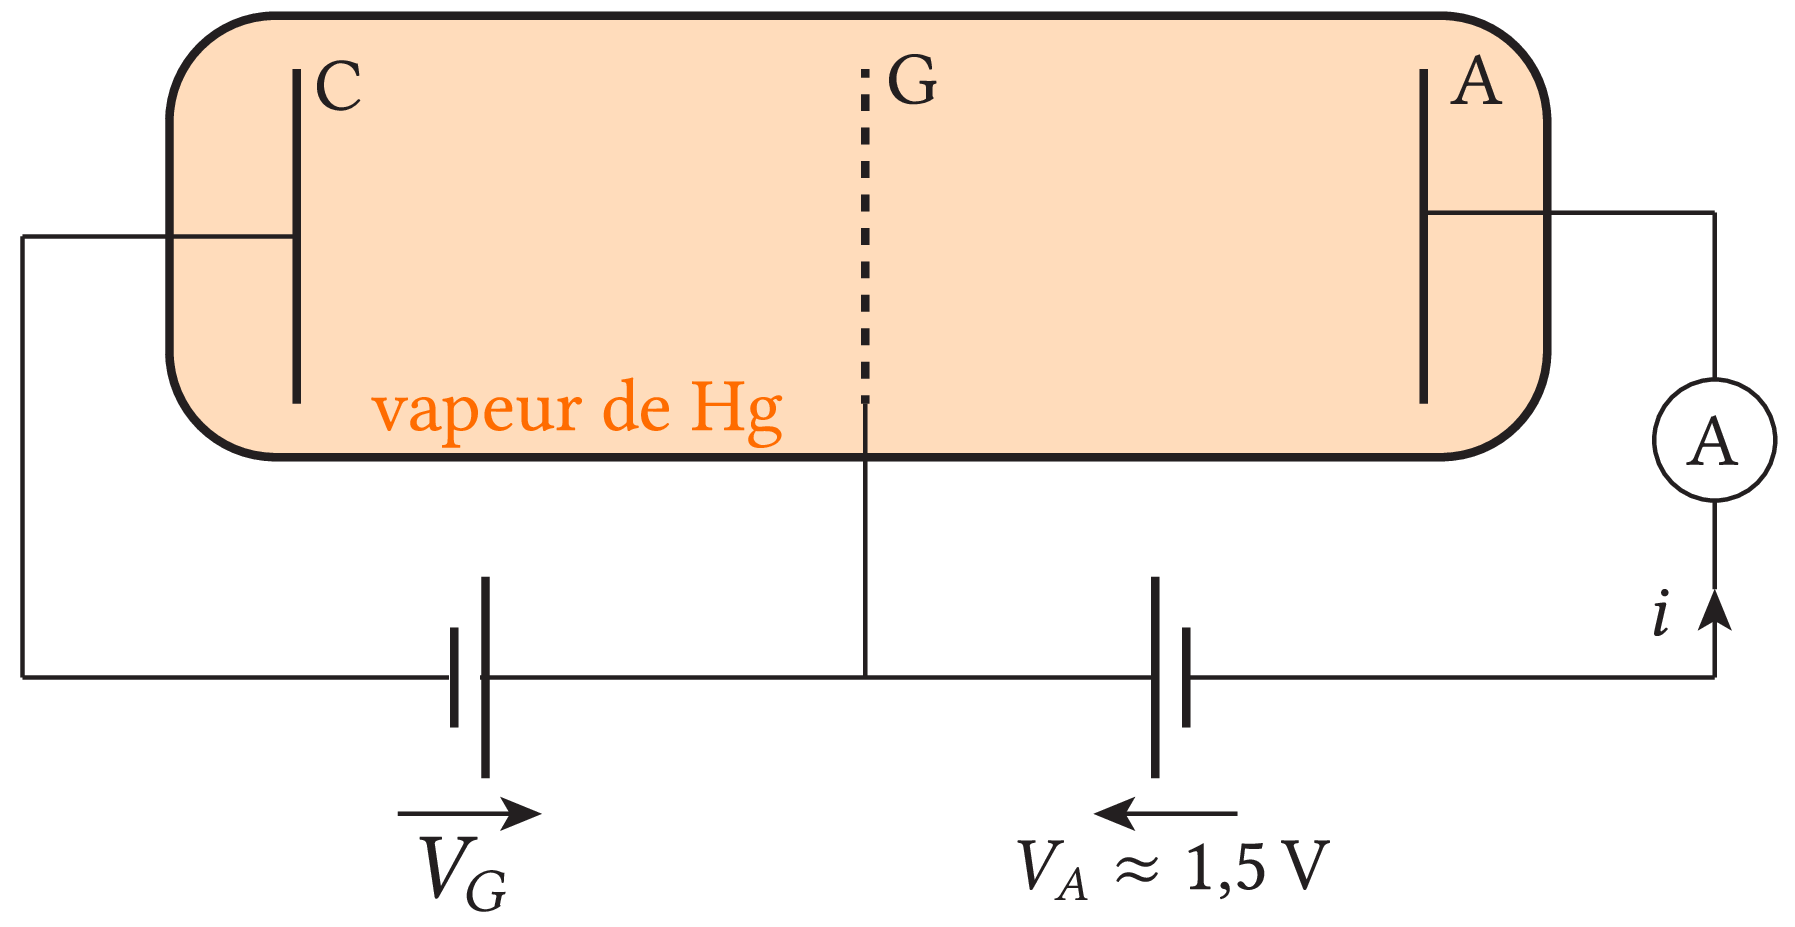
\includegraphics[width=0.49\linewidth]{Franck_Hertz_dispositif.png} 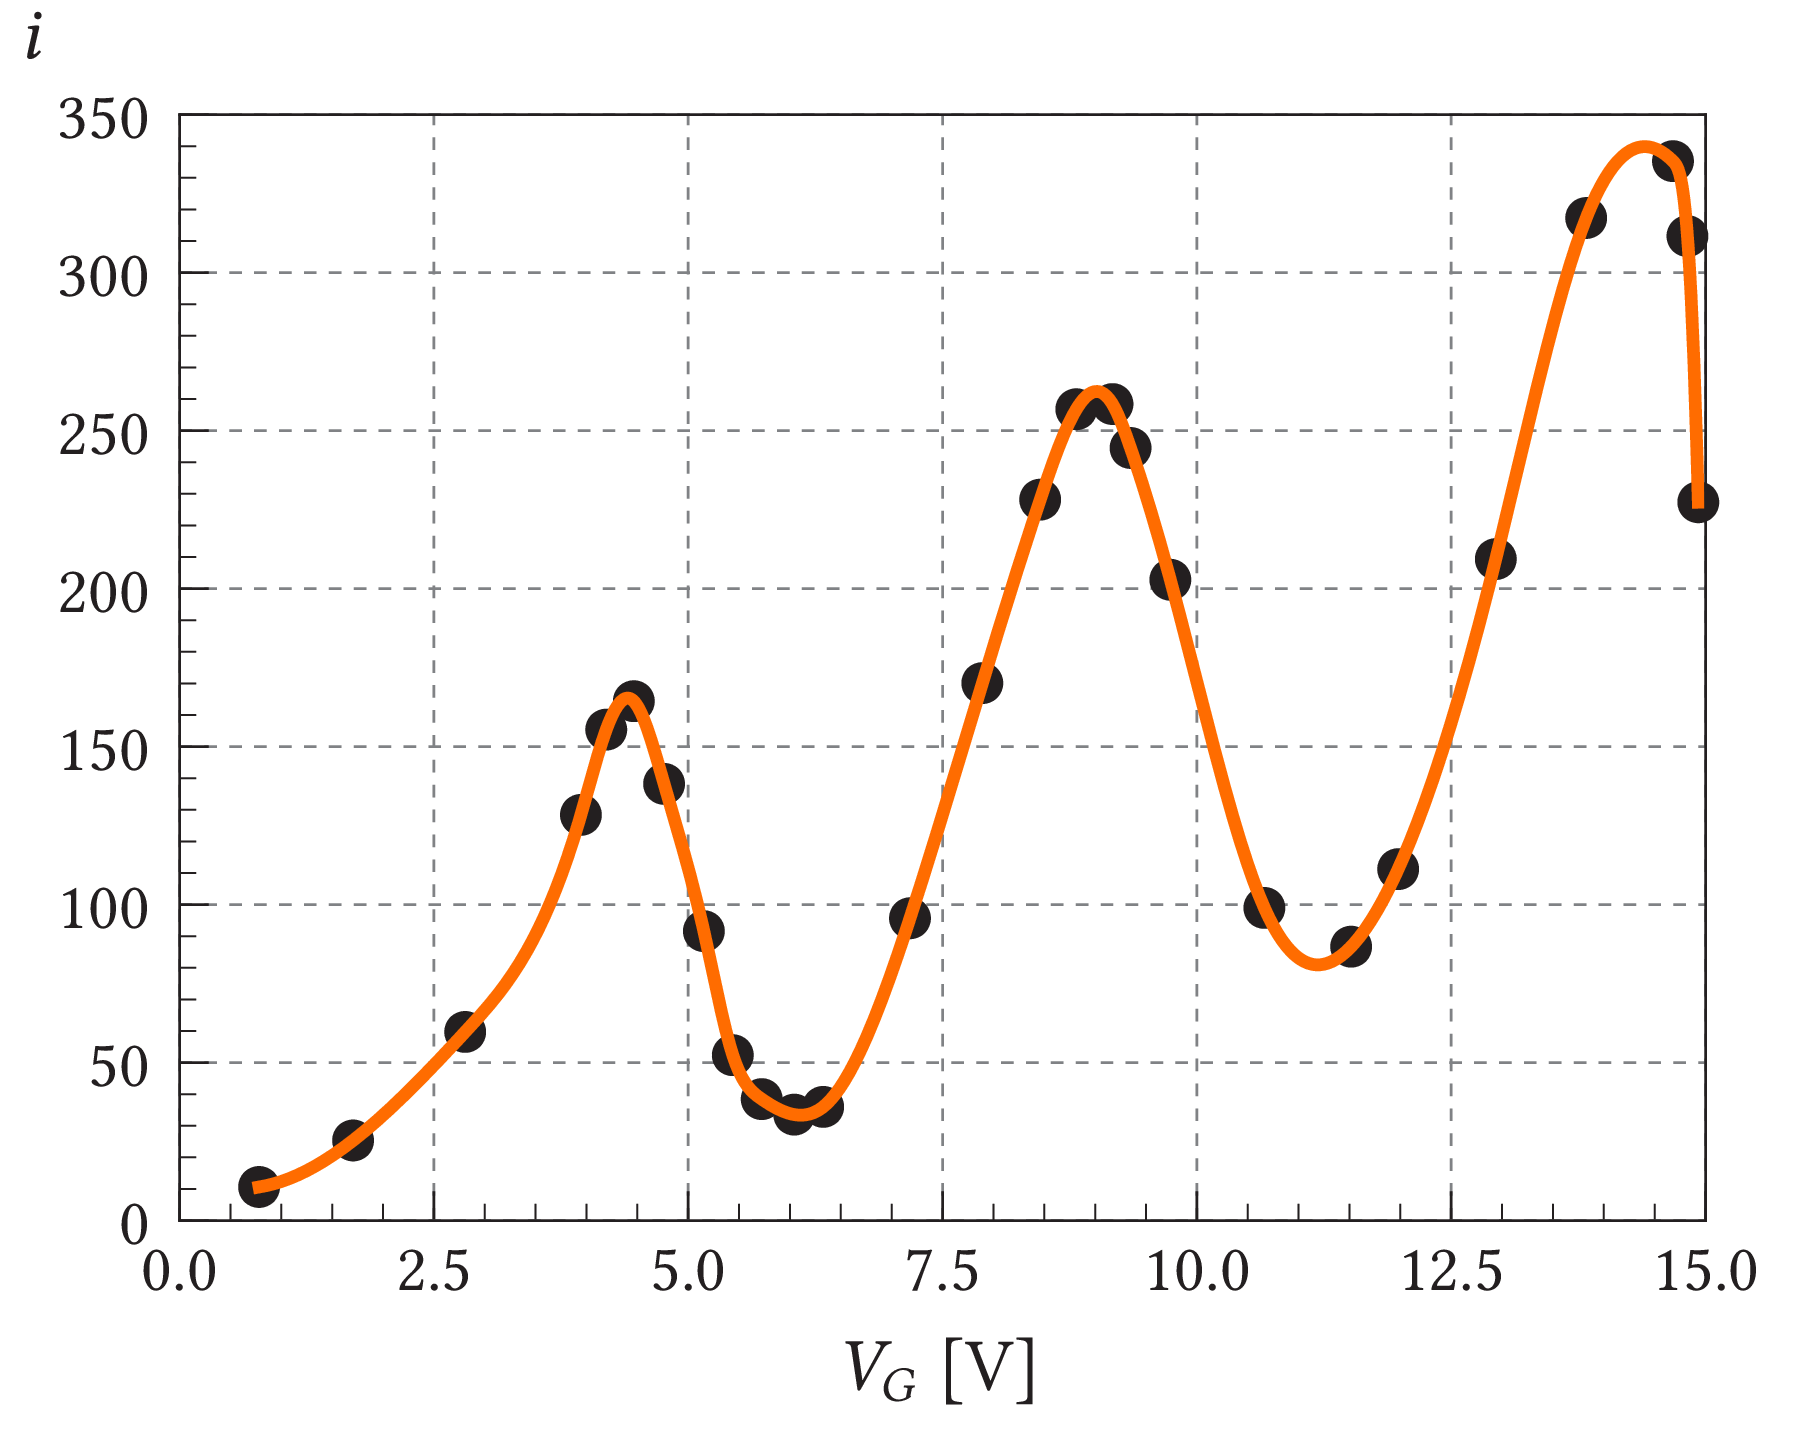
\includegraphics[width=0.49\linewidth]{Franck_Hertz_mesures.png}
	\caption{Expérience de Franck et Hertz. A gauche : dispositif de mesure. A droite : résultats de l'expérience. L'intensité mesurée $i$ est proportionnelle au nombre et à la vitesse des électrons (nous avons vu en cours $\vv j = - n e \vv v$). Elle est tracée en fonction du potentiel appliqué. Source : Froustey, Fillette et Roussille, \textit{Physique pour l'agrégation}.}
\end{figure}

Lorsqu'ils augmentent l'énergie cinétique des électrons, Franck et Hertz constatent que l'énergie des électrons qui sort de l'ampoule augmente aussi : rien d'anormal. Cependant, lorsque l'énergie des électrons dépasse 4.9\,eV, Franck et Hertz constatent que :
\begin{itemize}
	\item Les électrons sortants ont perdu quasiment toute leur énergie cinétique ;
	\item Les atomes de mercure émettent un rayonnement UV de longueur d'onde $\lambda_{\ce{Hg}} = 253.7$\,nm
\end{itemize}
Ces observations se reproduisent à chaque multiple de 4.9\,eV : les électrons subissent alors une chute de leur énergie cinétique, et les atomes de mercure émettent une lumière plus intense.

Or, on sait depuis longtemps, notamment à l'aide de la spectroscopie à réseau, que les atomes de mercure ont une raie d'émission à $\lambda_{\ce{Hg}}$. Donc, il semblerait que les électrons fournissent l'énergie nécessaire à l'atome de mercure pour émettre cette longueur d'onde. Cette expérience vient alors appuyer expérimentalement l'hypothèse formulée par Einstein pour expliquer l'effet photoélectrique : pour émettre une onde lumineuse, il faut disposer d'une quantité finie d'énergie. Et si l'on calcule cette énergie à partir de la formule d'Einstein $E = h c / \lambda$ et en utilisant la valeur de $h$ trouvée par Planck, on tombe sur : $E_{\ce{Hg}} = hc/\lambda_{\ce{Hg}} = 4.9$\,eV !

Cette expérience est la première confirmation expérimentale que l'énergie des atomes est quantifiée : lorsque l'électron impacte un atome, il lui permet de changer de niveau d'énergie, en passant de l'état fondamental à un état excité, dont l'énergie est supérieure de 4.9\,eV. En se désexcitant, l'atome de mercure émet alors un photon : c'est le processus inverse de l'effet photoélectrique.

Peut-on expliquer cette quantification de l'énergie à partir du formalisme de la mécanique quantique ondulatoire, c'est-à-dire en utilisant la fonction d'onde d'une particule ?

\subsection{Le puits de potentiel infini}

Nous allons dans la suite adopter un modèle extrêmement simplifié du comportement d'un électron dans un atome. L'électron est typiquement soumis à un potentiel électrostatique $V(r)$ qui présente un minimum en $r=0$. La forme de ce potentiel étant complexe (cf exercice sur le potentiel de Yukawa ; TD d'électrostatique), on va adopter une modélisation simpliste, mais est suffisant pour mettre en évidence la quantification de l'énergie : le puits de potentiel infini. 

\begin{definition}[Puits de potentiel infini]
	Le modèle du puits de potentiel infini de longueur $L$ correspond à un potentiel $V(x)$ ayant la forme suivante :
	\begin{align}
		V(x) &= 0 \quad \mathrm{pour} \quad 0 \le x \le L \\
		V(x) &= + \infty \quad \mathrm{sinon}
	\end{align}
\end{definition}

\begin{figure}[htbp]
	\centering 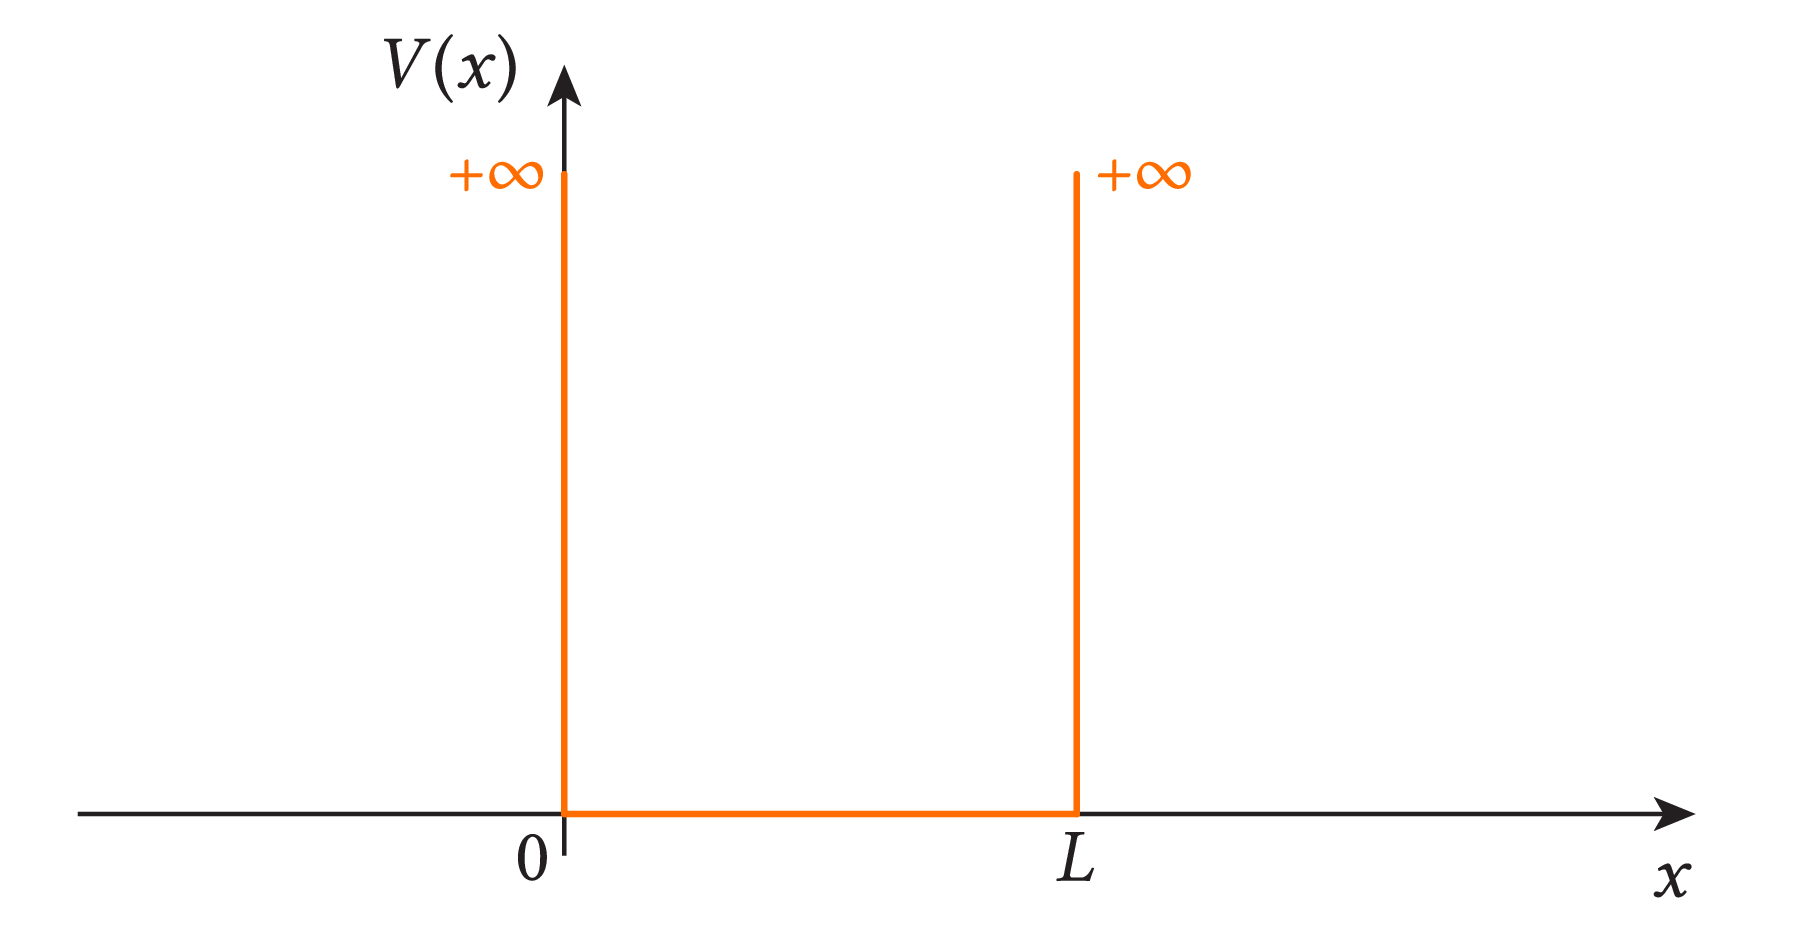
\includegraphics[width=0.5\linewidth]{Puits_infini.png}
	\caption{Puits de potentiel infini. Source : Froustey, Fillette et Roussille, \textit{Physique pour l'agrégation}.}
\end{figure}

Ici, $L$ va correspondre à la taille caractéristique de l'atome, de l'ordre de $10^{-10}$\,m.

Nous cherchons à déterminer les solutions possibles de l'équation de Schrödinger pour une particule quantique de masse $m$ qui y est confinée.

\subsection{Etats stationnaires}

Nous allons chercher dans un premier temps les fonctions d'onde qui satisfont cette équation sous forme d'états stationnaires :
\begin{definition}[Etat stationnaire]
	On appelle état stationnaire un état quantique caractérisé par une forme factorisée de la fonction d'onde, de la forme :
	\begin{equation}
		\psi(x,t) = \varphi(x) f(t)
	\end{equation}
	où $\varphi(x)$ et $f(t)$ sont des fonctions à valeurs complexes.
\end{definition}

\textbf{Attention !} Cette définition n'est pas analogue à la définition d'une onde stationnaire en physique classique. En effet, ici, les fonctions sont à valeurs complexes, alors que pour une onde stationnaire en mécanique classique elles sont à valeurs réelles. Typiquement, considérons la vibration lumineuse :
\begin{equation}
	\underline{s}(x,t) = e^{i\omega (t - x/c)} = e^{i \omega t} \times e^{i \omega x / c}
\end{equation}
Cette vibration lumineuse correspond évidemment à une onde propagative, et pourtant elle peut se mettre sous la forme d'un produit de deux fonctions complexes du temps et de l'espace.

\begin{proposition}
	Les états stationnaires ne sont pas forcément des ondes stationnaires au sens classique du terme.
\end{proposition}

Pourquoi appelle-t-on alors ces états des états stationnaires ? Ceci est lié à leur probabilité de présence.

\begin{capex}
	En exploitant la condition de normalisation, montrer que la probabilité de présence d'une particule dans un état stationnaire est indépendante du temps : $\rho_\mathbb{P}(x,t) = \rho_\mathbb{P}(x)$.
\end{capex}

\subsection{Equation de Schrödinger indépendante du temps}

Nous voulons désormais trouver les solutions de l'équation de Schrödinger qui sont des états stationnaires.

\begin{capex}
	Soit une particule dans un état stationnaire $\psi(x) = \varphi(x) f(t)$ soumise à un potentiel $V(x)$. A partir de la méthode de la séparation des variables, et en utilisant la condition de normalisation, déterminer les équations satisfaites par chacune des deux fonctions $f$ et $\varphi$.
\end{capex}

\begin{theorem}[Equation de Schrödinger indépendante du temps]
	La fonction d'onde d'un état stationnaire est de la forme :
	\begin{equation}
		\psi(x,t) = \varphi(x) \exp\left(-i \frac{E}{\hbar} t\right)
	\end{equation}
	où $E \in \mathbb{R}^+$ est l'énergie de la particule.
	La fonction $\varphi$ satisfait l'équation de Schrödinger indépendante du temps :
	\begin{equation}
		- \frac{\hbar^2}{2m} \frac{\dd^2 \varphi(x)}{\dd x^2} + V(x) \varphi(x) = E \varphi(x)
	\end{equation}
\end{theorem}

\begin{proposition}[Interprétation physique de l'équation de chrödinger indépendante du temps]
Il est possible d'apporter une interprétation physique à cette équation, qui indique la conservation de l'énergie :
\begin{itemize}
	\item $E$ correspond à l'énergie totale de la particule (analogue à l'énergie mécanique, en mécanique classique) ;
	\item $V(x)$ correspond à l'énergie potentielle de la particule ;
	\item Le terme $- \frac{\hbar^2}{2m} \frac{\dd^2 \varphi(x)}{\dd x^2}$ est donc relié à l'énergie cinétique de la particule.
\end{itemize}
\end{proposition}

\begin{remark}
	Le terme d'énergie cinétique devant être fini, la fonction $\varphi$ doit être dérivable deux fois sur $\mathbb{R}$. Ceci n'est pas le cas lorsque le potentiel $V(x)$ est infini : dans ce cas, $\varphi(x)$ est continue mais $\frac{\dd \varphi}{\dd x}$ peut être discontinue.
\end{remark}

\begin{capex}
	A partir de la forme des états stationnaires, retrouver la relation de Planck-Einstein. Est-elle vraie uniquement pour les photons ?
\end{capex}

\subsection{Etats stationnaires du puits de potentiel infini}

On cherche maintenant des états stationnaires pour une particule confinée dans un puits infini. Ils s'écrivent sous la forme :
\begin{equation}
        \psi(x,t) = \varphi(x) \exp\left(-i \frac{E}{\hbar} t\right)
\end{equation}
avec :
\begin{equation}
        - \frac{\hbar^2}{2m} \frac{\dd^2 \varphi(x)}{\dd x^2} + V(x) \varphi(x) = E \varphi(x)
\end{equation}

\begin{capex}
	Déterminer les conditions aux limites en $x=0$ et $x=L$, puis résoudre l'équation de Schrödinger et montrer que l'énergie de la particule est quantifiée.
\end{capex}

\begin{proposition}[Niveaux d'énergie d'une particule confinée dans un puits infini]
	Les états stationnaires d'une particule quantique dans un puits infini de taille $L$ sont les fonctions :
	\begin{equation}
		\psi_n(x,t) = \sqrt{\frac{2}{L}} \exp \left(-\frac{iE_nt}{\hbar}\right) \sin \left(\frac{n\pi}{L}\right)
	\end{equation}
	L'énergie est alors quantifiée :
	\begin{equation}
		E_n = n^2 \frac{\pi^2 \hbar^2}{2 m L^2}
	\end{equation}
	$n$ est appelé le nombre quantique d'un état propre, et la suite $(E_n)_{n \int \mathbb{N}^\ast}$ est appelé le spectre d'énergie de la particule quantique. Chaque valeur $E_n$ est un niveau d'énergie.
\end{proposition}

\begin{figure}[htbp]
	\centering 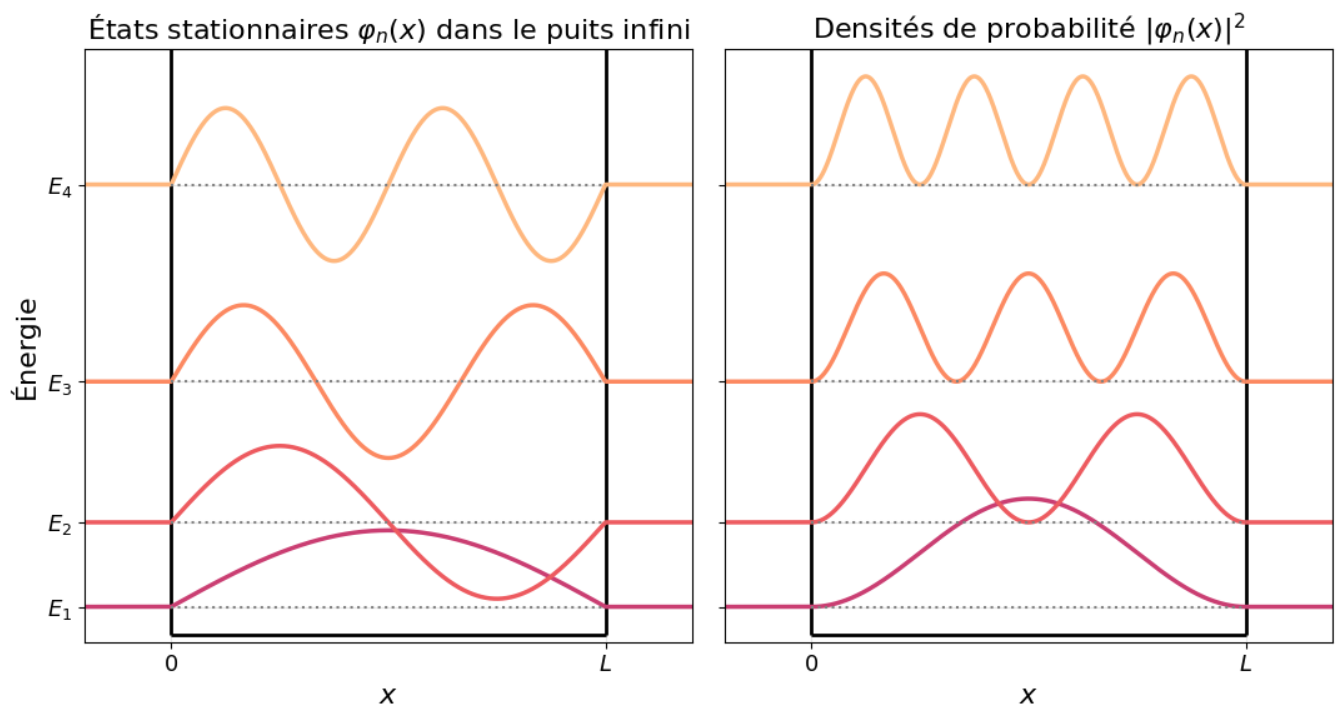
\includegraphics[width=0.9\linewidth]{puits_infini.png}
	\caption{Fonctions d'onde et probabilités de présence pour les quatre premiers états stationnaires. Conformément aux conventions habituelles en mécanique quantique, on a décalé la représentation graphique des fonctions d'onde verticalement pour faire coïncider le zéro de la fonction d'onde avec l'énergie du niveau concerné.}
\end{figure}

La densité de probabilité de présence $|\varphi(x)|^2$ dans les premiers états stationnaires est représentée sur la partie droite de la figure ci-dessus. On peut y constater que :
\begin{itemize}
	\item Cette densité n'est jamais uniforme : dans un état stationnaire, on observe notamment des noeuds où la probabilité de présence de la particule est nulle.
	\item L'état de nombre quantique $n$ présente $n+1$ noeuds, de manière générale l'énergie d'un état stationnaire augmente avec le nombre de noeuds.
\end{itemize}

\begin{capex}
	Proposer une analogie formelle entre la corde de Melde vue en MPSI et le puits de potentiel infini en mécanique quantique.
\end{capex}

\subsection{Puits de potentiel fini ou de forme quelconque}

Ces propriétés sont toujours vraies dans le cas d'un puits de potentiel fini et/ou de forme quelconque, on peut notamment le vérifier à partir de simulations numériques. Dans ce cas, cependant, on observe deux différences majeures :
\begin{itemize}
	\item On n'a plus de condition aux limites de la forme $\varphi=0$ aux bords du puits de potentiel, donc la fonction d'onde déborde en dehors du puits de potentiel. La particule a donc une probabilité non nulle de se trouver à des endroits où son énergie est inférieure à l'énergie potentielle ! Nous aborderons cet aspect en détail dans le prochain chapitre de mécanique quantique.
	\item Si le puits de potentiel est de taille finie, alors il existe un nombre fini d'états stationnaires. C'est notamment le cas dans les atomes : le nombre quantique principal $n$ ne peut prendre qu'un nombre fini de valeurs (qui dépend de la ligne du tableau périodique dans laquelle on se trouve).
\end{itemize}

\begin{figure}[htbp]
	\centering 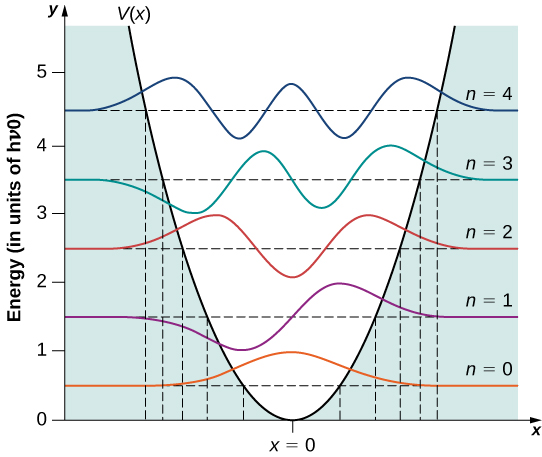
\includegraphics[width=0.5\linewidth]{fonctions_oscillateur_harmonique.jpg}
	\caption{Exemple des solutions de l'équation de Schrödinger dans un puits de potentiel correspondant à un oscillateur harmonique : l'énergie est quantifiée, mais les fonctions d'onde débordent dans la zone où $V(x)>E$. Pour les plus curieux.ses, ces fonctions correspondent aux polynômes d'Hermite. Source : LibreTexts Physique.}
\end{figure}

\section{Energie de confinement}

\subsection{Energie de confinement du puits infini}

Intéressons-nous au niveau d'énergie le plus bas possible d'une particule confinée dans un puits de potentiel, $n=1$ :
\begin{definition}[Etat fondamental]
	L'état stationnaire d'une particule quantique confinée correspondant au niveau d'énergie le plus bas est appelé état fondamental.
\end{definition}

Dans le cas d'une particule quantique dans un puits de potentiel infini, on trouve :
\begin{equation}
	E_1 = \frac{\pi^2 \hbar^2}{2 m L^2}
\end{equation}
On peut remarquer que, dans le cas du puits de potentiel infini, la probabilité que la particule soit sur le segment $x \in [0,L]$ est égale à 1, et dans ce segment on a uniformément $V(x) = 0$. Ainsi, l'énergie potentielle de la particule est nulle et $E_1$ correspond à son énergie cinétique. On en conclut que dans le niveau fondamental, l'énergie cintétique de la particule est non nulle. Ce résultat est en contradiction avec la mécanique classique qui prévoit qu'à l'équilibre, la particule est immobile, l'énergie cinétique est nulle, et la position correspond au minimum d'énergie potentielle.

\begin{definition}[Energie de confinement]
	On appelle énergie de confinement d'une particule son énergie dans l'état fondamental, en prenant pour référence le minimum de l'énergie potentielle. Dans un système quantique, l'énergie de confinement est strictement positive.
\end{definition}

\subsection{Principe d'indétermination de Heisenberg}

\begin{capex}
	Exploiter la relation $E \ge E_1$ pour obtenir une inégalité entre la quantité de mouvement de la particule, $p$, et la largeur $L$ du puits de potentiel.
\end{capex}

Cette inégalité traduit en fait une propriété fondamentale de la matière en mécanique quantique : on ne peut pas mesurer avec une précision arbitraire à la fois la position et la vitesse d'une particule. Autrement dit, la variance des lois de probabilité $\rho_\mathbb{P}(x)$ de la position de la particule $x$, et de l'impulsion de la particule $p$ sont reliées par une inégalité :
\begin{theorem}[Inégalité de Heisenberg spatiale]
	Il existe une limitation intrinsèque à la définition simultanée de la position et de la quantité de mouvement d'une particule :
	\begin{equation}
		\Delta x \times \Delta p \ge \frac{\hbar}{2}
	\end{equation}
\end{theorem}

\subsection{Application à un puits de forme quelconque : l'atome d'hydrogène}

Considérons désormais un puits de potentiel de forme quelconque. Typiquement, on peut étudier la position de l'électron dans l'atome d'hydrogène, dont le potentiel est de la forme :
\begin{equation}
	V(r) = - \frac{e^2}{4 \pi \epsilon_0 r}
\end{equation}

\begin{capex}
	En utilisant l'inégalité de Heisenberg, déterminer l'ordre de grandeur du rayon $a_0$ de l'atome d'hydrogène dans son état fondamental.
\end{capex}

\begin{remark}
	On constate ici qu'à l'aide de la mécanique quantique, on est capable de prédire théoriquement la taille d'un atome, ce qui n'était pas possible avec la mécanique classique ! Il s'agit de l'un des grands succès de cette théorie.
\end{remark}

\section{Etats non stationnaires d'une particule quantique confinée}

\subsection{Superposition d'états stationnaires}

Jusqu'ici, nous avons considéré uniquement des états stationnaires dans un puits de potentiel. Que se passe-t-il si l'on étudie une combinaison linéaire d'états stationnaires ? 

On reprend l'exemple du puits de potentiel infini, et on considère par une particule qui se trouve dans une superposition des états 1 et 3 :
\begin{equation}
	\psi(x,t) = \frac{1}{\sqrt{2}} \psi_1(x,t) + \frac{1}{\sqrt{2}} \psi_3(x,t)
\end{equation}
\begin{capex}
	Etablir la densité de probabilité de présence associée à la particule. Quelle propriété remarquable constate-t-on ?
\end{capex}

Cette propriété se généralise à toute somme d'états stationnaires (pas uniquement dans le cas du puits infini).
\begin{proposition}
	La superposition de deux états stationnaires d'énergie $E_a$ et $E_b \neq E_a$ n'est pas un état stationnaire. La densité de probabilité de présence, en tout point de l'espace, est une fonction sinusoïdale du temps de pulsation :
	\begin{equation}
		\omega = \frac{|E_a - E_b|}{\hbar}
	\end{equation}
\end{proposition}
\begin{demonstration}
	\textit{La démonstration n'est pas à connaître. Elle est cependant intéressante car tout à fait analogue à la démonstration de la formule de Fresnel en optique.} Supposons que l'on a deux états stationnaires $\Psi_a$ et $\Psi_b$, on peut alors écrire, par propriété des états stationnaires :
	\begin{equation}
		\Psi_a(x,t) = \varphi_a(x) \exp\left(-i\frac{E_a t}{\hbar}\right) \quad \mathrm{et} \quad \Psi_b(x,t) = \varphi_b(x) \exp\left(-i\frac{E_b t}{\hbar}\right)
	\end{equation}
	Alors on peut considérer une superposition de ces états :
	\begin{equation}
		\Psi(x,t) = \alpha \Psi_a(x,t) + \beta \Psi_b(x,t)
	\end{equation}
	où les coefficients $\alpha$ et $\beta$ sont choisis de sorte à avoir une fonction d'onde normalisée. 
	Cette superposition correspond à la densité de probabilité :
	\begin{align}
		\rho_{\mathbb{P}}(x,t) &= | \alpha \Psi_a(x,t) + \beta \Psi_b(x,t) |^2 \\
		&= |\alpha \Psi_a(x,t)|^2 + |\beta \Psi_b(x,t)|^2 + 2 \Re \left( \alpha \Psi_a(x,t) \beta^\ast \Psi_b(x,t)^\ast \right) \\
		&= |\alpha \varphi_a(x)|^2 + |\beta \varphi_b(x)|^2 + 2 \Re \left( \alpha \varphi_a(x) \beta^\ast \varphi_b(x)^\ast \exp\left( i \frac{(E_b - E_a)t}{\hbar} \right) \right) \\
		&= A(x) + B(x) \cos \left( \frac{E_b-E_a}{\hbar} t + \theta(x) \right)
	\end{align}
	où l'on a posé $A(x) = |\alpha \varphi_a(x)|^2 + |\beta \varphi_b(x)|^2$ et $B(x) e^{i\theta(x)} = 2 \alpha \varphi_a(x) \beta^\ast \varphi_b(x)^\ast$. On constate effectivement que la superposition des états a une probabilité de présence qui varie dans le temps.
\end{demonstration}

\subsection{Relation temps-énergie de Heinseberg (hors-programme mais parfois utile)}

On constate ainsi que, lorsqu'une indétermination $\Delta E$ est présente sur l'énergie de la particule (par exemple lors d'une superposition d'états d'énergie différente), on a des variations temporelles de la probabilité de présence de la particule avec un temps caractéristique $\tau$ de l'ordre de $\frac{\hbar}{\Delta E}$.

Cette observation traduit une relation plus générale :
\begin{proposition}[Relation temps-énergie de Heisenberg]
	Un système quantique évoluant dans le temps avec un temps caractéristique $\tau$ a son énergie affectée d'une indétermination quantique $\Delta E$ telle que :
	\begin{equation}
		\tau \times \Delta E \sim \hbar
	\end{equation}
\end{proposition}







\end{document}
